\let\negmedspace\undefined
\let\negthickspace\undefined
\documentclass[journal]{IEEEtran}
\usepackage[a5paper, margin=10mm, onecolumn]{geometry}
%\usepackage{lmodern} % Ensure lmodern is loaded for pdflatex
\usepackage{tfrupee} % Include tfrupee package

\setlength{\headheight}{1cm} % Set the height of the header box
\setlength{\headsep}{0mm}     % Set the distance between the header box and the top of the text
\usepackage{multicol}
\usepackage{gvv-book}
\usepackage{gvv}
\usepackage{cite}
\usepackage{amsmath,amssymb,amsfonts,amsthm}
\usepackage{algorithmic}
\usepackage{graphicx}
\usepackage{textcomp}
\usepackage{xcolor}
\usepackage{txfonts}
\usepackage{listings}
\usepackage{enumitem}
\usepackage{mathtools}
\usepackage{gensymb}
\usepackage{comment}
\usepackage[breaklinks=true]{hyperref}
\usepackage{tkz-euclide} 
\usepackage{pgfplots}
\pgfplotsset{compat=1.18}
\usepackage{listings}
% \usepackage{gvv}                                        
\def\inputGnumericTable{}                                 
\usepackage[latin1]{inputenc}                                
\usepackage{color}                                            
\usepackage{array}                                            
\usepackage{longtable}                                       
\usepackage{calc}                                             
\usepackage{multirow}                                         
\usepackage{hhline}                                           
\usepackage{ifthen}                                           
\usepackage{lscape}
\usepackage{tikz}
% Marks the beginning of the document
\begin{document}
\bibliographystyle{IEEEtran}
\vspace{3cm}

\title{NCERT-10.3.4.1.1}
\author{EE24BTECH11056 - S.Kavya Anvitha}
\maketitle
%\newpage
\bigskip

\renewcommand{\thefigure}{\theenumi}
\renewcommand{\thetable}{\theenumi}
\section*{Problem:}
Solve the system of linear equations:
\[
x + y = 5 \quad \text{(1)}
\]
\[
2x - 3y = 4 \quad \text{(2)}
\]

\section*{Step 1: Represent the system in matrix form}
The system of equations can be written as:
\[
A \mathbf{x} = \mathbf{b}
\]
where
\[
A = \begin{pmatrix} 1 & 1 \\ 2 & -3 \end{pmatrix}, \quad \mathbf{x} = \begin{pmatrix} x \\ y \end{pmatrix}, \quad \mathbf{b} = \begin{pmatrix} 5 \\ 4 \end{pmatrix}.
\]

\section*{Step 2: Perform LU Decomposition}
We decompose the matrix \(A\) into the product of a lower triangular matrix \(L\) and an upper triangular matrix \(U\), i.e., 
\[
A = LU
\]
where
\[
L = \begin{pmatrix} 1 & 0 \\ l_{21} & 1 \end{pmatrix}, \quad U = \begin{pmatrix} u_{11} & u_{12} \\ 0 & u_{22} \end{pmatrix}.
\]

Now, let's compute the LU decomposition step by step.

First, we find the elements of \(U\) and \(L\):
\[
u_{11} = a_{11} = 1, \quad u_{12} = a_{12} = 1.
\]
Next, we compute \(l_{21}\) and \(u_{22}\):
\[
l_{21} = \frac{a_{21}}{u_{11}} = \frac{2}{1} = 2,
\]
\[
u_{22} = a_{22} - l_{21} u_{12} = -3 - 2 \times 1 = -5.
\]
So the LU decomposition is:
\[
L = \begin{pmatrix} 1 & 0 \\ 2 & 1 \end{pmatrix}, \quad U = \begin{pmatrix} 1 & 1 \\ 0 & -5 \end{pmatrix}.
\]

\section*{Step 3: Solve for \(\mathbf{x}\) using \(LU\) decomposition}
Now we solve the system in two steps using forward substitution and backward substitution.

First, solve \(L \mathbf{y} = \mathbf{b}\) for \(\mathbf{y}\):
\[
\begin{pmatrix} 1 & 0 \\ 2 & 1 \end{pmatrix} \begin{pmatrix} y_1 \\ y_2 \end{pmatrix} = \begin{pmatrix} 5 \\ 4 \end{pmatrix}.
\]
This gives:
\[
y_1 = 5, \quad 2y_1 + y_2 = 4 \quad \Rightarrow \quad 2(5) + y_2 = 4 \quad \Rightarrow \quad y_2 = -6.
\]
Thus, \(\mathbf{y} = \begin{pmatrix} 5 \\ -6 \end{pmatrix}\).

Next, solve \(U \mathbf{x} = \mathbf{y}\) for \(\mathbf{x}\):
\[
\begin{pmatrix} 1 & 1 \\ 0 & -5 \end{pmatrix} \begin{pmatrix} x \\ y \end{pmatrix} = \begin{pmatrix} 5 \\ -6 \end{pmatrix}.
\]
This gives:
\[
-5y = -6 \quad \Rightarrow \quad y = \frac{6}{5}.
\]
\[
x + y = 5 \quad \Rightarrow \quad x + \brak{\frac{6}{5}} = 5 \quad \Rightarrow \quad x = \frac{19}{5},
\]

Thus, the solution is \(x = \frac{19}{5}\) and \(y = \frac{6}{5}\).

\section*{LU Decomposition using Doolittle's algorithm}
The LU decomposition can be efficiently compted using Doolittle's algorithm. This method generates the matrices \( L \) (lower triangular) and \( U \) (upper triangular) such that \( A = LU \). The elements of these matrices are calculated as follows: \\
Elements of the \( U \) Matrix:  \\
For each column \( j \):
\begin{align}
	U_{ij} &= A_{ij} \quad \text{if } i = 0, \\
	U_{ij} &= A_{ij} - \sum_{k=0}^{i-1} L_{ik} U_{kj} \quad \text{if } i > 0.
\end{align}
Elements of the \( L \) Matrix: \\
For each row \( i \):
\begin{align}
	L_{ij} &= \frac{A_{ij}}{U_{jj}} \quad \text{if } j = 0, \\
	L_{ij} &= \frac{A_{ij} - \sum_{k=0}^{j-1} L_{ik} U_{kj}}{U_{jj}} \quad \text{if } j > 0.
\end{align}

This systematic approach ensures that the matrix \( A \) is decomposed into \( L \) and \( U \) without requiring row swaps, provided \( A \) is nonsingular.
\begin{figure}[h!]
   \centering
   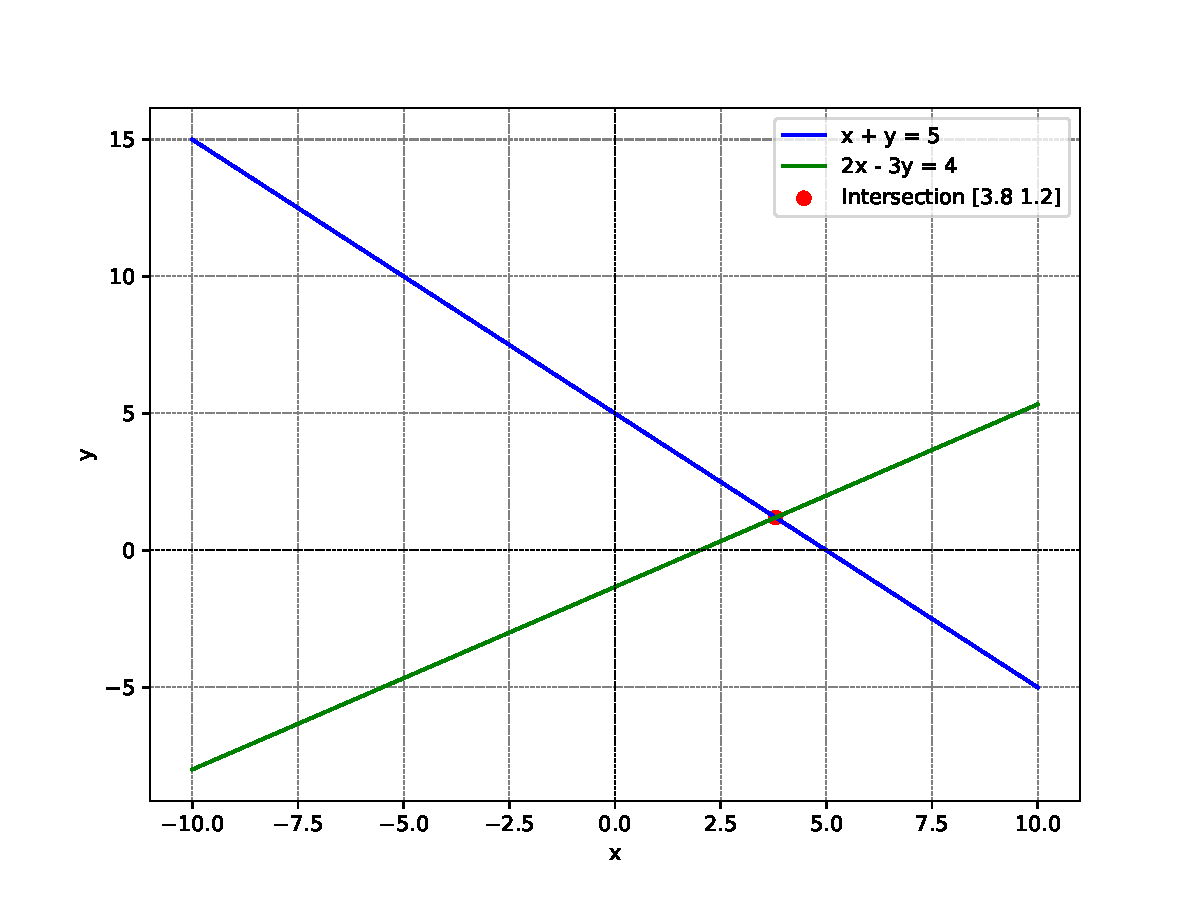
\includegraphics[width=\columnwidth]{figs/fig.pdf}
\end{figure}
\end{document}
